% !TEX root = main.tex

This paper is about \emph{relative expressiveness} results for 
\emph{higher-order process calculi}, core programming languages that 
integrate name- and process-passing in communications.
We focus on calculi coupled with \emph{session types} that denote interaction protocols. 
%The expressivity relations that we aim to are essential for the transference of reasoning techniques, notably behavioral equivalences, across different typed languages. 
%Our motivation for studying expressivity relations is to establish a firm foundation for the transference of reasoning techniques, notably behavioral equivalences, across different session typed languages. 
%Our results %of relative expressiveness 
%enable us to identify 
Expressiveness results allows us to 
%Our goal is to 
identify
a \emph{core %process language % concurrency %with session primitives, 
calculus}
that encompasses both first- and higher-order session communication.
%equally expressive as several other
%calculi with sessions.
%\emph{essential} constructs, i.e., constructs those not expressible in terms of other constructs. 
%They are also central ingredients in the   \emph{transference of reasoning techniques}, notably behavioral theories, across different languages.
Establishing such results 
in our typed setting 
is challenging because 
%Since session types denote protocols, 
 it entails defining 
 not only a translation 
relating source and target languages (\emph{encoding}), but also a translation 
relating their associated session types. 
We aim at a very particular class of correct encodings: namely \emph{fully abstract} and \emph{type-preserving} encodings.
%This is a challenging task, as we elaborate next.
Next, we elaborate on our aims,   approach, and contributions.

\jparagraph{Context}
In \emph{session-based concurrency}, concurrent interactions are organized into \emph{sessions}, basic communication units.
Interaction patterns can then be abstracted as expressive \emph{session types}~\cite{honda.vasconcelos.kubo:language-primitives}, against which process specifications may be checked. 
%These patterns are defined as %(possibly recursive) 
%sequences of communication actions: % (send/receive a value, offer/select a behavior).
%For instance, 
%session type $T_1 = \btinp{\mathsf{str}} \btout{\mathsf{int}}  \tinact$ may be intuitively read as: receive (?) a value of type $\mathsf{str}$,then output (!) a value of type $\mathsf{int}$, finally close the protocol.
Session type $\btinp{U} S$ (resp.  $\btout{U} S$)
describes a protocol that first receives (resp. sends) a value of type $U$ and then continues as protocol $S$.
Also, given an index set $I$, types $\btbra{l_i:S_i}_{i \in I}$ 
and $\btsel{l_i:S_i}_{i \in I}$ 
define %, respectively,
%a branching and selection constructs for  
 a labeled choice mechanism; types 
$\trec{t}{S}$ 
and 
$\tinact$ denote recursive and completed protocols, respectively.
%describes a protocol that offers
%(resp. ) 
%Type $\tinact$ denotes the completed protocol.
In the (first-order) $\pi$-calculus~\cite{MilnerR:calmp1}, 
session types describe the intended interactive behavior of the names/channels in a process.
%names/channels are endowed with session types (such as $T_1$) representing their intended interactive behavior.
Session-based concurrency has also been casted in \emph{higher-order} process
calculi which, by combining features from the $\lambda$-calculus and the $\pi$-calculus, 
enable the exchange of values that may contain processes~\cite{tlca07,DBLP:journals/jfp/GayV10}. 
Besides offering a natural bridge between concurrent and functional computation, 
higher-order calculi with sessions enable the specification of protocols involving \emph{code mobility}, 
frequent in practice.
In the main higher-order session language  studied here (denoted \HOp),
 values in communications include names but also (first-order) abstractions---functions from name identifiers to processes. 
 %(In contrast, higher-order abstractions---functions from processes to processes---are disallowed.)
 (In contrast, we rule out functions from processes to processes, i.e., higher-order abstractions.)
Abstractions can be linear or shared; their types are  denoted $\lhot{C}$ and $\shot{C}$, respectively ($C$ 
%is a first-order type $C$ (say, a session name).
denotes a name). We may have a 
session type such as, e.g.,
%$T_2 = \btbra{upload:\btinp{\lhot{\mathsf{int}}}\tinact ~ , ~ sha:\btinp{\shot{\mathsf{int}}}\tinact}_{}$
$$S = \btbra{up:\btinp{\lhot{C}}\btout{\mathsf{ok}}\tinact ~ , ~ down:\btout{\shot{C}}\btout{\mathsf{ok}}\tinact ~ , ~quit:\btout{\mathsf{bye}}\tinact}_{}$$
that abstracts a server that offers different behaviors to clients: 
%  clients to select among distinct  behaviors: %namely, 
  to \emph{upload} a linear function, % (to be received by the server), 
  to \emph{download} a shared function, % (to be sent by the server),
   or to \emph{quit} the protocol. Subsequently, 
  the server sends a message ($\mathsf{ok}$ or $\mathsf{bye}$) before closing the session.



 

\jparagraph{The Problem}
%Roughly speaking, 
  \HOp %, a higher-order process language that 
extends Sangiorgi's higher-order $\pi$-calculus~\cite{SangiorgiD:expmpa} with session primitives.
To be precise, %More precisely, 
\HOp
includes
constructs for 
%session establishment
synchronisation along shared names, 
session communication (value passing, labelled choice) along linear names,
recursion, 
 (first-order) abstractions %(i.e., functions from name identifiers  to processes)
 and applications.
% (denoted $\lambda x.P$ and $(\lambda x.P)a$, resp.).
%While synchronization on shared names (useful to model session establishment) is 
%non deterministic, session communication is deterministic and occurs on linear names.
\HOp is therefore a rather rich language. This begs the question:
%\begin{quote}
is there a \emph{sub-calculus} of \HOp with equal expressivity? %hich is as expressive as the whole calculus? 
%\end{quote}
This question is of foundational interest, 
for reasoning/validation techniques are more easily developed on small formalisms. 
It also has practical ramifications, 
as such a \emph{core calculus} could be taken as reference in 
the design of %(functional) 
programming languages with session types support.
%implementations of languages with session primitives.
Expressivity results may then help justifying useful connections 
between foundational and practical advances on languages with concurrency and communication.

%We have recently developed a behavioral theory  for \HOp~\cite{characteristic_bis}:
%we introduced
%\emph{characteristic bisimilarity}, a sound and complete 
%characterization of contextual equivalence. % that enables tractable analyses.


\jparagraph{Approach}
%Previous studies already suggest 
It is known
that first- and higher-order com\-mu\-ni\-cation %---the paradigms that uniformly coexist in \HOp---
independently constitute 
the main sources 
of expressivity in \HOp. %: \emph{name passing} and constructs for \emph{infinite behavior} (i.e., recursion and replication). 
On the one hand, the expressivity of name-passing calculi (untyped and typed) is well known; e.g., the $\pi$-calculus can express 
%the $\lambda$-calculus and 
process-passing calculi~\cite{SangiorgiD:expmpa}. 
%In the $\pi$-calculus, recursion and replication can be expressed in terms of each other. 
On the other hand, higher-order concurrency is itself quite expressive: 
even  calculi without name passing and recursion are known to be Turing equivalent~\cite{DBLP:journals/iandc/LanesePSS11}.
Also, in higher-order calculi,
recursion/replication operators are redundant, as they can be represented using process passing and duplication~\cite{ThomsenB:plachoasgcfhop}. 
%For these reasons, 
%Consequently, 
Based on these observations, 
in this paper we study the expressivity of \HOp in relation to two  sub-calculi
that distill the essence of first- and higher-order session-based concurrency:
\begin{enumerate}[-]
\item the session \sessp-calculus \jpc{(denoted~\sessp)}: \HOp without abstractions and applications;
\item the \HO-calculus: \HOp without recursion and name passing.
\end{enumerate}
%Interestingly, %\HO and \sessp distil the essence of higher- and first-order session-based concurrency:
We assess the expressivity 
 of \HOp, \HO, and \sessp as delineated by session types. 
We establish strong correspondences between 
these calculi via 
type-preserving, fully abstract encodings (up to 
behavioural equalities)---see \figref{fig:express}. 
While \sessp is, 
in essence, the calculus in~\cite{honda.vasconcelos.kubo:language-primitives}, 
%this paper shows 
our \emph{main discovery} is 
that \HO  is a new core calculus 
for %higher-order 
session concurrency.
%\figref{fig:express} summarises %our expressivity 
%our encodability results. 


%While encoding \HOp 
%into the $\pi$-calculus preserving session types 
%(extending  known  results for untyped processes~\cite{SangiorgiD:expmpa}) is 
%%\jpc{already}
%significant, 



\jparagraph{Contributions}
Our main contribution is 
an encoding of \HOp into \HO (\secref{subsec:HOpi_to_HO}).  
Since \HO lacks 
both name-passing and recursion, this encoding involves two key challenges:
\begin{enumerate}[a.]
\item In known (typed) 
encodings of name-passing into process-passing~\cite{SaWabook} %are limited: % in that 
%they come with restrictions on name usages;  
%they 
%work for %name-passing 
%calculi 
%with \emph{capability types} 
%in which 
only the output capability of names can be sent---a received name cannot be used in later inputs.
This is far too limiting in \HOp, where 
 session names %denoting arbitrary protocols 
 may be passed around (\emph{delegation})
and types describe interaction  \emph{structures}, rather than ``loose'' name capabilities. % at a given time.

\begin{figure}[t]
\centering
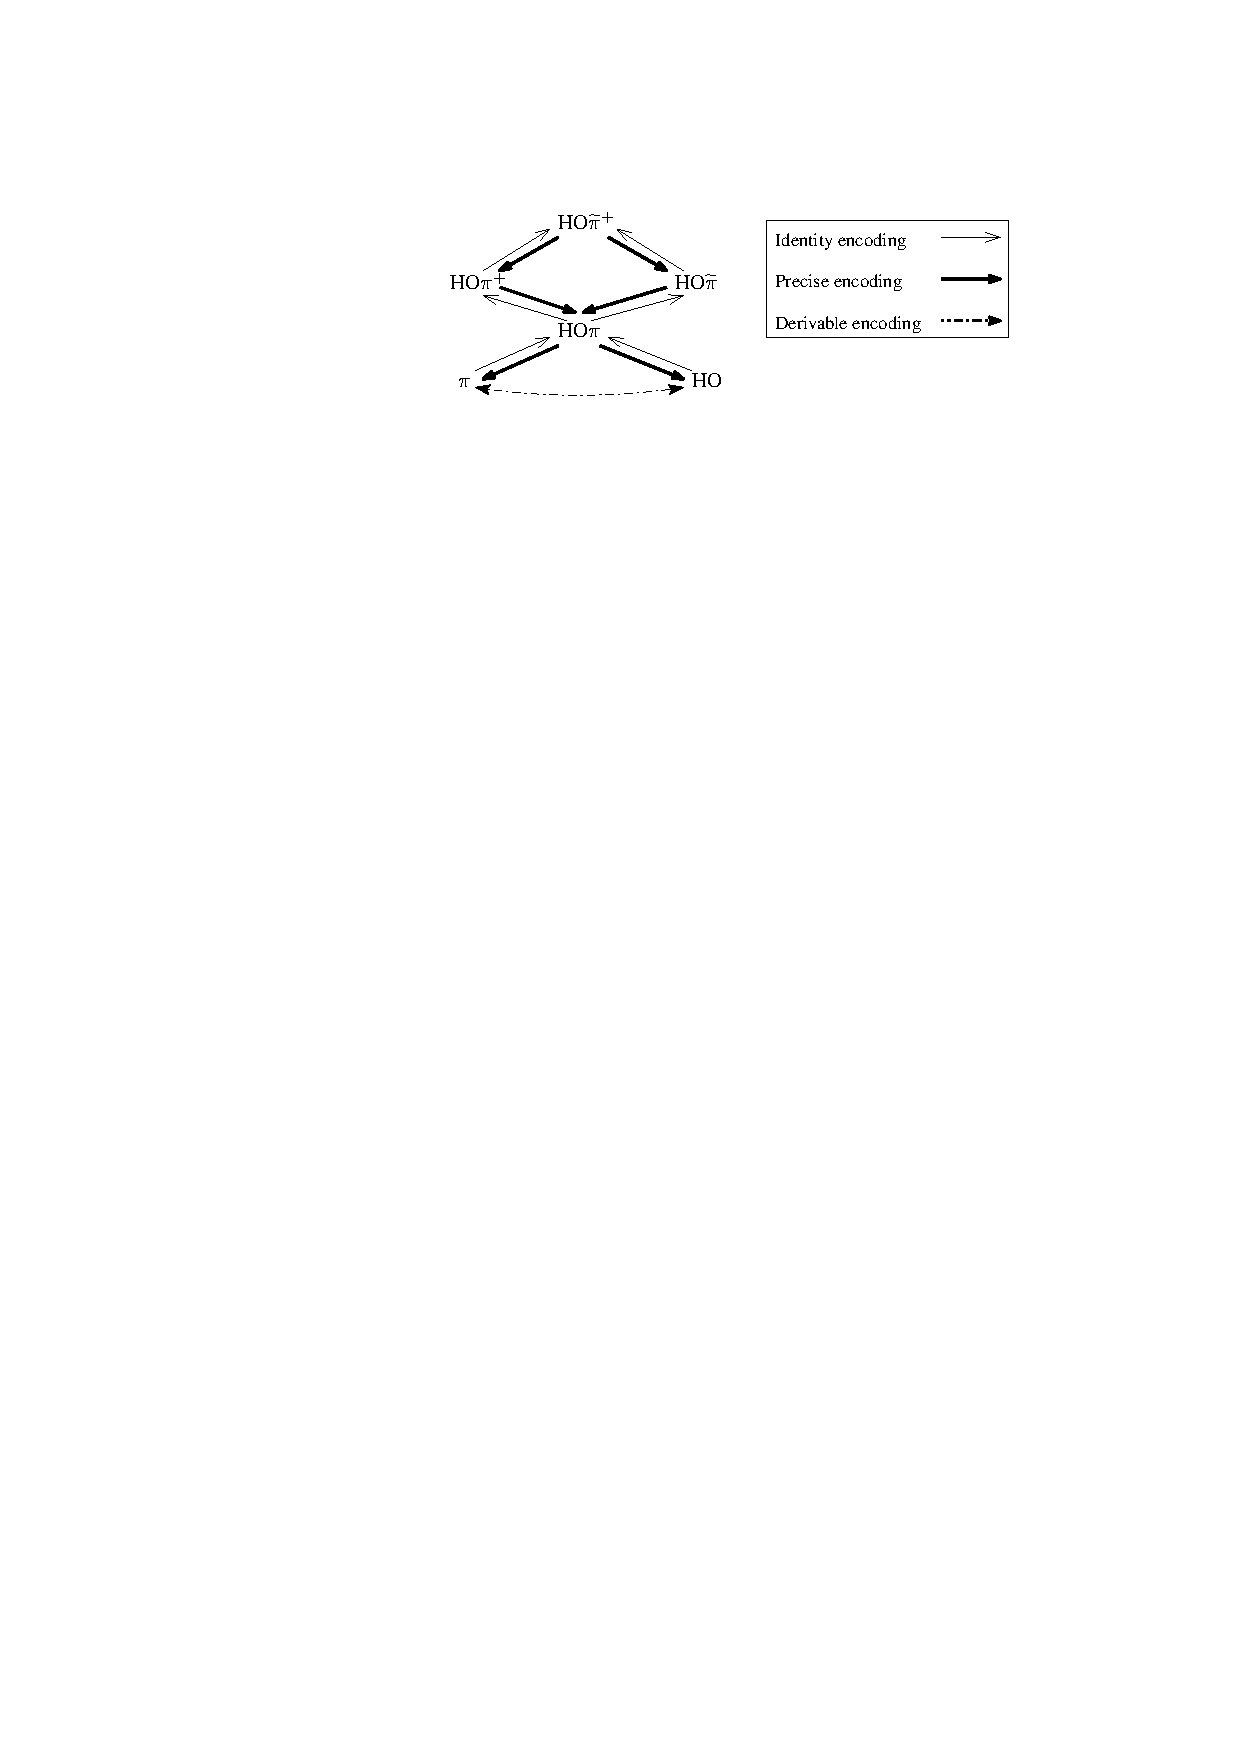
\includegraphics[scale=1]{diag.pdf}

	\caption{Encodability in Higher-Order Sessions. 
	Precise encodings are defined in \defref{def:goodenc}.
	\label{fig:express}}
\vspace{-5mm}
\Hlinefig
\end{figure}

\item %As mentioned above, recursion % and replication)
%can be encoded in untyped higher-order calculi using process duplication. Unfortunately, this kind of encodings 
Known encodings of recursion in untyped higher-order calculi
do not carry over to session typed calculi such as \HOp,
because linear abstractions cannot be copied/duplicated. Hence, the discipline of session types  limits 
the possibilities for representing infinite behaviors---even simple forms, such as input-guarded replication.
\end{enumerate}




%MOTIVATION FIRST ENCODING (). \emph{Still to highlight: recursive type required, no recursion, small example.

%--- 
\noi
%We illustrate our approach. % to these challenges.
Our encoding overcomes these two obstacles, as we discuss in the following section.

Additional technical contributions include: (i)~the encodability of \HO into \sessp (\secref{subsec:HOp_to_sessp}); (ii)~a non encodability result showing that shared names strictly add expressive power to session calculi (\secref{ss:negative});
(iii)~extensions of our encodability results to richer settings (\secref{sec:extension}). 
In essence, (i) extends known  results for untyped processes~\cite{SangiorgiD:expmpa} to the session typed setting.
Although (ii) may be somewhat expected, to our knowledge we are the first to offer a proof of this separation result, 
exploiting session determinacy and typed equivalences.
Finally, concerning (iii), we develop extensions of our encodings to 
\begin{enumerate}[-]
\item The extension of \HOp with \emph{higher-order} abstractions (\HOpp); 
\item The extension of \HOp with polyadic name passing and abstraction (\pHOp); 
\item The super-calculus of \HOpp and \pHOp (\PHOpp), equivalent to the calculus in~\cite{tlca07}.
\end{enumerate}
%\figref{fig:express} summarises %our expressivity 
%our encodability results. 
%From a global standpoint, our 
These
encodability results connect \HOp with existing higher-order process calculi~\cite{tlca07}, and  
further highlight the status of \HO as the core calculus for session concurrency.




\jparagraph{Outline} 
%This paper  is structured as follows.
%\begin{enumerate}[$\bullet$]
\secref{sec:overview} overviews key ideas of our encodability results.
%\item 
\secref{sec:calculus} presents the higher-order session calculus \HOp, its 
subcalculi \HO and \sessp, and extensions.  
It also summarizes the session type system
and states type soundness for \HOp and its variants.
\secref{s:expr} defines \emph{precise (typed) encodings} by extending encodability criteria 
 for
untyped processes~(e.g.~\cite{DBLP:journals/iandc/Gorla10,DBLP:conf/icalp/LanesePSS10}).
%\item 
\secref{sec:positive} %and \S\,\ref{sec:negative}
gives encodings of \HOp into \HO and of \HOp into~\sessp.
These encodings 
are shown to be \emph{precise} (Thms.~\ref{f:enc:hopitoho} and~\ref{f:enc:hotopi}).
Mutual encodings between \sessp and \HO are derivable; 
all these calculi are thus equally expressive.
%Exploiting determinacy and typed equivalences,
We also prove the non-encodability of shared names
into linear names (\thmref{t:negative}).
%\item
\secref{sec:extension} studies extensions of \HOp: 
we show that both \HOpp 
%(the extension with higher-order applications) 
and \pHOp 
%(the extension with polyadicity) 
are encodable in \HOp
(Thms.~\ref{f:enc:hopiptohopi} and \ref{f:enc:phopiptohopi}).
%This connects our work to the existing higher-order session calculus in~\cite{tlca07} (here denoted  $\PHOpp$).
%\item 
\secref{sec:relwork} concludes with related works. 
The paper is self-contained. 
{\bf\em Additional related work, more examples, omitted definitions, and  proofs 
%can be found
are 
in~\cite{KouzapasPY15}.} 

